\documentclass[letterpaper, twoside, 10pt]{report}

\usepackage{fontspec}
\usepackage{listings}
\usepackage{graphicx}
\usepackage[
		letterpaper,
		marginparwidth={8em}
		]{geometry}
\usepackage{microtype}
\usepackage{titlesec}
\usepackage{fancyref}
\usepackage{framed}
\usepackage{float}
\usepackage[dvipsnames,prologue]{xcolor}
\graphicspath{ {images/} }

%%%%% FLOATS %%%%%
\newfloat{program}{tbphH}{lop}[section]
\floatname{program}{Program}

%%%%% TITLE DEFINITION %%%%%
\title{k-OS System Manual}
\author{Headquarters, Kerbal Space Center}
\date{\today}

%%%%% DOCUMENT %%%%%
\begin{document}

%%%%% TITLE PAGE %%%%%
\begin{titlepage}
\begin{center}
		\fboxsep10pt
		\colorbox{gray}{\begin{minipage}{6.5in}
		\begin{flushright}
		\texttt{\LARGE{\textbf{ KM\,03-62}}}\\
		\texttt{\large KERBAL SYSTEMS FIELD MANUAL}
		\vfill
		\end{flushright}
		\end{minipage}}
		\texttt{\Huge KERBAL OPERATING SYSTEM}
		\vfill
	\end{center}
\end{titlepage}

%%%%% LIST OF EFFECTIVE PAGES %%%%%

%%%%% TABLE OF CONTENTS %%%%%
\tableofcontents

%%%%% CONTENT INCLUSION %%%%%
\part{Introduction}
	\section*{k-OS and KerboScript}
		KerboScript is the language used to program the CPU device attached to your vessel and kOS is the operating system that interprets the code you write. The program can be as simple as printing the current altitude of the vessel and as complicated as a six-axis autopilot controller taking your vessel from the launchpad to Duna and back! With kOS, the sky is not the limit.
		This mod is compatible with RemoteTech, you just have to make sure you copy the program onto the local CPU before it goes out of range of KSC.
	\section*{Installation}
		Like other mods, simply merge the contents of the zip file into your Kerbal Space Program folder.
	\section*{KerboScript}
		KerboScript is a programming language that is derived from the language of planet Kerbin, which sounds like gibberish to non-native speakers but for some reason is written exactly like English. As a result, KerboScript is very English-like in its syntax. For example, it uses periods as statement terminators.
		The language is designed to be easily accessible to novice programmers, therefore it is case-insensitive, and types are cast automatically whenever possible.
		A typical command in KerboScript might look like this:
			
			\begin{lstlisting}[frame=single,language=XML]
			PRINT "Hello World"}
			\end{lstlisting} 
\part{Tutorials}
	\section{Quick Start}
		This is a quick start guide for the Kerbal Operating System (kOS). It is intended for those who are just starting with using kOS. It does presume you have played Kerbal Space Program before and know the basics of how to fly a rocket under manual control. It does NOT assume you know a lot about computer programming, and it will walk you through some basic first steps.
		\subsection{First example: Hello World}
In the grand tradition of programming tutorials, the first example will be how to make a script that does nothing more than print the words ?Hello World? on the screen. The purpose of this example is to show where you should put the files, how to move them about, and how to get one to run on the vessel.

\paragraph{Step 1: Start a new sandbox-mode game}
(You can use kOS in a career mode game, but it requires a part that you have to research which isn?t available at the start of the tech tree, so this example will just use sandbox mode to keep it simple.)

\paragraph{Step 2: Make a vessel in the Vehicle Assembly Bay}
Make the vessel contain any unmanned command core, a few hundred units of battery power, a means of recharging the battery such as a solar panel array, and the ?Comptronix CX-4181 Scriptable Control System?. (From this point onward the CX-4181 Scriptable Control System part will be referred to by the acronym ?SCS?.) The SCS part is located in the parts bin under the ?Control? tab (the same place where RCS thrusters and Torque Wheels are found.)

\begin{center}
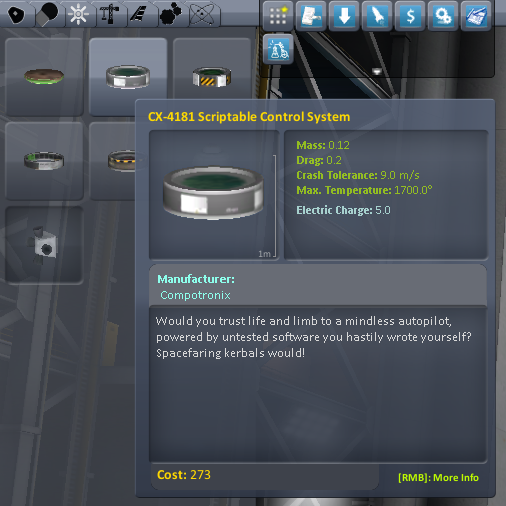
\includegraphics[width=3in]{SCS_parts_bin}
\end{center}

\paragraph{Step 3: Put the vessel on the launchpad}
Put the vessel on the launchpad. For this first example it doesn?t matter if the vessel can actually liftoff or even has engines at all.

\paragraph{Step 4: Invoke the terminal}
Rightclick for the SCS part on the vessel and then click the button that says ?Open Terminal?.

Note that if the terminal is semi-transparent, this means it?s not currently selected. If you click on the terminal, then your keyboard input is directed to the terminal INSTEAD of to piloting. In other words if you type W A S D, you?ll actually get the word ?wasd? to appear on the terminal, rather than the W A S D keys steering the ship. To switch back to manual control of the game instead of typing into the terminal, click outside the terminal window anywhere on the background of the screen.

\paragraph{Step 5: See what an interactive command is like}
You should now see an old-school looking text terminal like the one shown below. Type the line:

\begin{lstlisting}[frame=single,language=XML]
CLEARSCREEN. PRINT "==HELLO WORLD==".
\end{lstlisting} 

into the terminal (make sure to actually type the periods (?.?) as shown) and hit ENTER. Note that you can type it in uppercase or lowercase. kOS doesn?t care.

\begin{center}
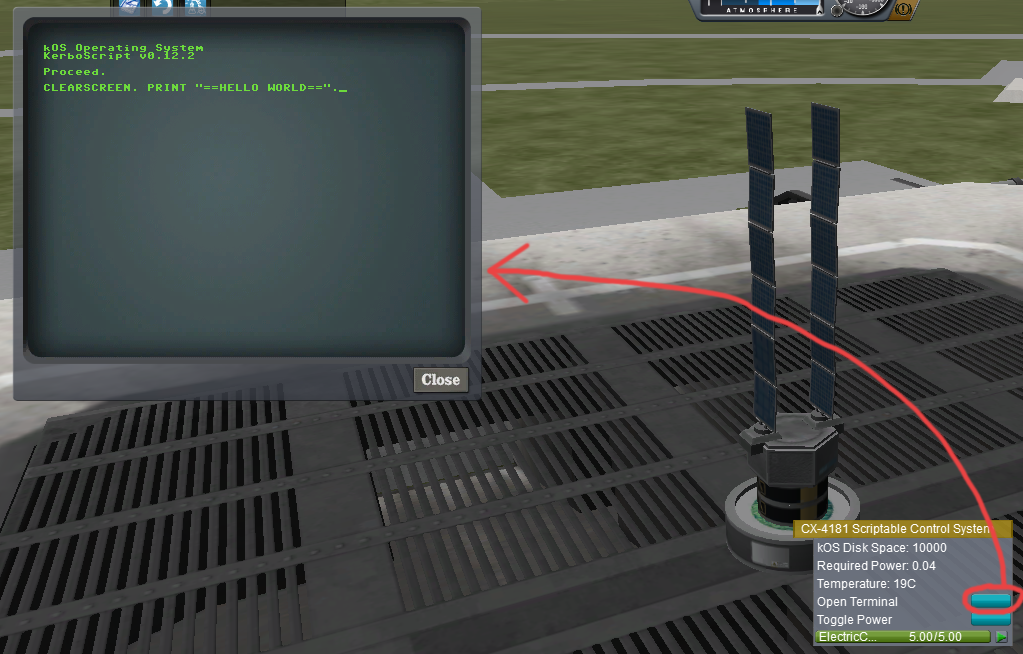
\includegraphics[width=3in]{terminal_open_1}
\end{center}

The terminal will respond by showing you this:

\begin{center}
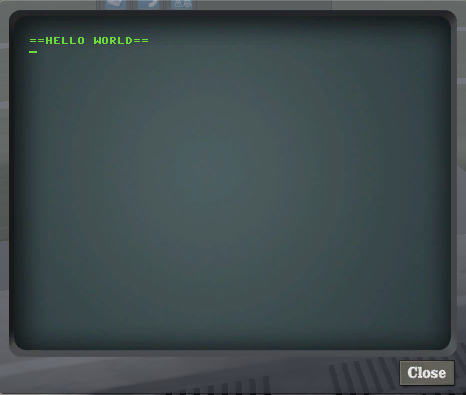
\includegraphics[width=3in]{terminal_open_2}
\end{center}

\paragraph{Step 6: Okay that?s great, but how can you make that happen in a program script instead?}
Like so: Enter this command:

\begin{lstlisting}[frame=single,language=XML]
EDIT HELLO.
\end{lstlisting} 

(Don?t forget the period (?.?). All commands in kOS are ended with a period. Again, you can type it in uppercase or lowercase. kOS doesn?t care.)

You should see an editor window appear, looking something like this (without the text inside because you?re starting a blank new file):

\begin{center}
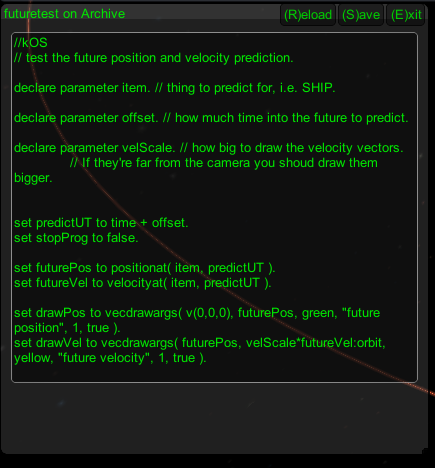
\includegraphics[width=3in]{editor}
\end{center}

Type this text into the window:

\begin{lstlisting}[frame=single,language=XML]
PRINT "=========================================".
PRINT "      HELLO WORLD".
PRINT "THIS IS THE FIRST SCRIPT I WROTE IN kOS.".
PRINT "=========================================".
\end{lstlisting} 

Click ?Save? then ?Exit? in the editor popup window.

Side Note: The editor font - Experienced programmers may have noticed that the editor?s font is proportional width rather than monospaced and that this is not ideal for programming work. You are right, but there is little that can be done about it for a variety of technical reasons that are too complex to go into right now.
Then on the main text terminal Enter:

\begin{lstlisting}[frame=single,language=XML]
RUN HELLO.
\end{lstlisting} 

And you will see the program run, showing the text on the screen like so.

\begin{center}
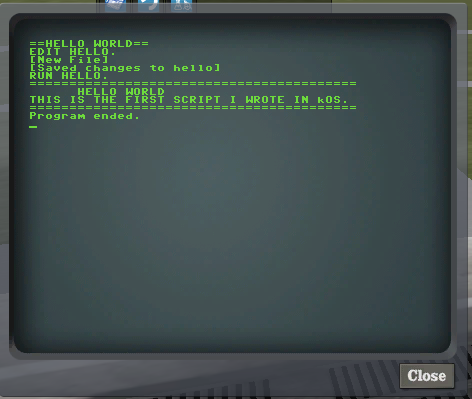
\includegraphics[width=3in]{hello_world1}
\end{center}

\paragraph{Step 7: Okay, but where is this program?}
To see where the ?HELLO? program has been saved, Issue the command LIST FILES like this:

\begin{lstlisting}[frame=single,language=XML]
LIST FILES.
\end{lstlisting} 

(Note, that the default for the LIST command is to list FILES, so you can leave the word ?FILES? off if you like.)

It should look like this, showing you the HELLO program you just wrote:

\begin{center}
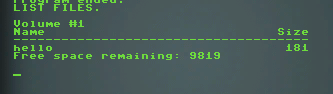
\includegraphics[width=3in]{hello_list.png}
\end{center}

This is a list of all the files on the currently selected VOLUME. By default, when you launch a new vessel, the currently selected VOLUME is called ?1? and it?s the volume that?s stored on THAT SCS part that you are running all these commands in.

This is the local volume of that SCS part. Local volumes such at this tend to have very small limited storage, as you can see when you look at the space remaining in the list printout.

If you?re wondering where the file is stored physically on your computer, it?s represented by a section inside the persistence file for your saved game, as a piece of data associated with the SCS part. This is important because it means you can?t access the program from another vessel, and if this vessel ever crashes and the SCS part explodes, then you?ve lost the program.

\paragraph{Step 8: I don?t like the idea that the program is stored only on this vessel. Can?t I save it somewhere better? }More permanent?
Yes. Yes you can.

There is another VOLUME that always exists called the Archive, which is also referred to as volume 0. (either name can be used in commands). The archive is conceptually stored somewhere back at Kerbin home base in the Space Center rather than on your vessel. It has infinite storage space, and does not disappear when your vessel is gone. ALSO, it actually exists across saved games - if you launch one saved game, put a new file in the Archive, and then later launch a different saved game, that file will be there in that game too.

To use the Archive, first we?ll have to introduce you to a new command, called SWITCH TO. The SWITCH TO command changes which VOLUME is the one that you are doing your work with.

To work with the archive, and create a second ?hello world? file there, you issue these commands and see what they do:

\begin{lstlisting}[frame=single,language=XML]
SWITCH TO 0.
EDIT HELLO2. // Make a new file here that just says: PRINT "hi again".
LIST FILES.
RUN HELLO2.
SWITCH TO 1.
LIST FILES.
RUN HELLO.
\end{lstlisting} 

But where is it stored behind the scenes? The archive is currently slightly violating the design of KSP mods that puts everything in the GameData folder. The kSP Archive is actually stored in the Ships/Script folder of your MAIN KSP home, not inside GameData.

If a file is stored inside the archive, it can actually be edited by an external text editor of your choice instead of using kOS?s in-game editor. This is usually a much better practice once you start doing more complex things with kOS. You can also make new files in the archive folder. Just make sure that all the files end with a .ks file name suffix or kOS won?t use them.	

Further reading about files and volumes:

Volumes
File Control
File Information		
		\subsection{Second Example: Doing something real}%%%%% Next Section %%%%%
Okay that?s all basic setup stuff but you?re probably clamoring for a real example that actually does something nifty.

This example will show the crudest, most basic use of kOS just to get started. In this example we?ll make a program that will launch a vessel using progressively more and more complex checks. kOS can be used at any stage of a vessel?s flight - launching, circularizing, docking, landing,... and in fact launching is one of the simpler piloting tasks that you can do without much need of automation. Where kOS really shines is for writing scripts to do touchy sensitive tasks like landing or docking or hovering. These are the areas that can benefit from the faster reaction speed that a computer script can handle.

But in order to give you an example that you can start with from scratch, that?s easy to reload and retry from an initial point, we?ll use an example of launching.

\paragraph{Step 1: Make a vessel}
Make any sort of rocket that can lift you to orbit that fills the following pattern:

It uses ONLY liquid fuel rockets. The example code here will assume this is the case. kOS can deal with solid fuel boosters as well, but to keep the example simple we?ll use liquid fuel only here.
Make the vessel?s staging list set up in the right order for a launch. (Make sure it has no need to manually rightclick parts to stage things weirdly, and no need to use action groups to activate stages weirdly).
Make sure the vessel has plenty of torque power to stay steady without a lot of wobble.
Make the vessel have at least these parts on it:
battery power of at least 400 charge
ability to recharge equal to at least 6 solar panel sections or 1 RTG unit
the kOS SCS part somewhere in the stack, near the top bit where it won?t fall off due to staging.
Step 2: Make the start of the script
Okay, so type the lines below in an external text editor of your choice (i.e. Notepad on Windows, or TextEdit on Mac, or whatever you fancy):

\begin{lstlisting}[frame=single,language=XML]
// My First Launcher.

PRINT "Counting down:".
FROM {local countdown is 10.} UNTIL countdown = 0 STEP {SET countdown to countdown - 1.} DO {
    PRINT "..." + countdown.
    WAIT 1. // pauses the script here for 1 second.
}
\end{lstlisting} 

See those things with the two slashes (?//?)? Those are comments in the kerboscript language and they?re just ways to write things in the program that don?t do anything - they?re there for humans like you to read so you understand what?s going on. In these examples you never actually have to type in the things you see after the slashes. They?re there for your benefit when reading this document but you can leave them out if you wish.

Save the file in your Ships/Script folder of your KSP installation under the filename ?hellolaunch.ks?. DO NOT save it anywhere under GameData/kOS/. Do NOT. According to the KSP standard, normally KSP mods should put their files in GameData/[mod name], but kOS puts the archive outside the GameData folder because it represents content owned by you, the player, not content owned by the kOS mod.

By saving the file in Ships/Script, you have actually put it in your archive volume of kOS. kOS will see it there immediately without delay. You do not need to restart the game. If you do:

\begin{lstlisting}[frame=single,language=XML]
SWITCH TO 0.
LIST FILES.
\end{lstlisting} 

after saving the file from your external text editor program, you will see a listing of your file ?hellolaunch? right away. Okay, now copy it to your local drive and give it a try running it from there:

\begin{lstlisting}[frame=single,language=XML]
SWITCH TO 1.
COPY HELLOLAUNCH FROM 0.
RUN HELLOLAUNCH.
\end{lstlisting} 

\begin{center}
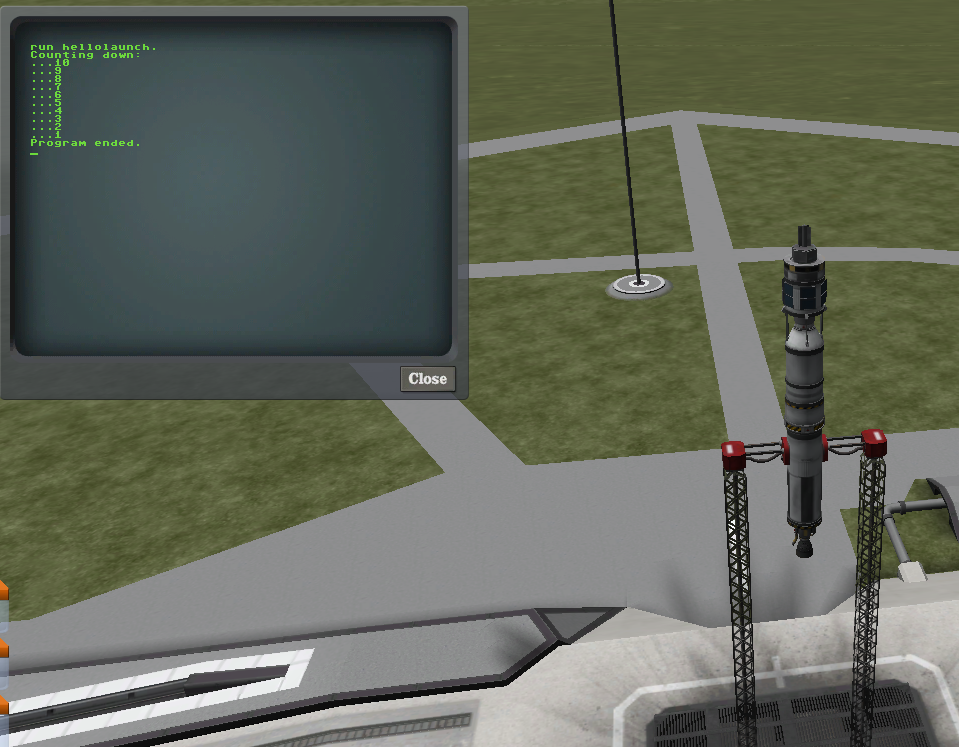
\includegraphics[width=3in]{example_2_1.png}
\end{center}

Okay so the program doesn?t actually DO anything yet other than just countdown from 10 to 0. A bit of a disappointment, but we haven?t written the rest of the program yet.

You?ll note that what you?ve done is switch to the local volume (1) and then copy the program from the archive (0) to the local volume (1) and then run it from the local volume. Technically you didn?t need to do this. You could have just run it directly from the archive. For those looking at the KSP game as a bit of a role-play experience, it makes sense to never run programs directly from the archive, and instead live with the limitation that software should be copied to the craft for it to be able to run it.

\paragraph{Step 3: Make the script actually do something}
Okay now go back into your text editor of choice and append a few more lines to the hellolaunch.ks file so it now looks like this:

\begin{lstlisting}[frame=single,language=XML]
// My First Launcher.

PRINT "Counting down:".
FROM {local countdown is 10.} UNTIL countdown = 0 STEP {SET countdown to countdown - 1.} DO {
    PRINT "..." + countdown.
    WAIT 1. // pauses the script here for 1 second.
}

PRINT "Main throttle up.  2 seconds to stabalize it.".
LOCK THROTTLE TO 1.0.   // 1.0 is the max, 0.0 is idle.
WAIT 2. // give throttle time to adjust.
UNTIL SHIP:MAXTHRUST > 0 {
    WAIT 0.5. // pause half a second between stage attempts.
    PRINT "Stage activated.".
    STAGE. // same as hitting the spacebar.
}
WAIT UNTIL SHIP:ALTITUDE > 70000. // pause here until ship is high up.

// NOTE that it is vital to not just let the script end right away
// here.  Once a kOS script just ends, it releases all the controls
// back to manual piloting so that you can fly the ship by hand again.
// If the pogram just ended here, then that would cause the throttle
// to turn back off again right away and nothing would happen.
\end{lstlisting} 

Save this file to hellolaunch.ks again, and re-copy it to your vessel that should still be sitting on the launchpad, then run it, like so:

\begin{lstlisting}[frame=single,language=XML]
COPY HELLOLAUNCH FROM 0.
RUN HELLOLAUNCH.
\end{lstlisting} 

\begin{center}
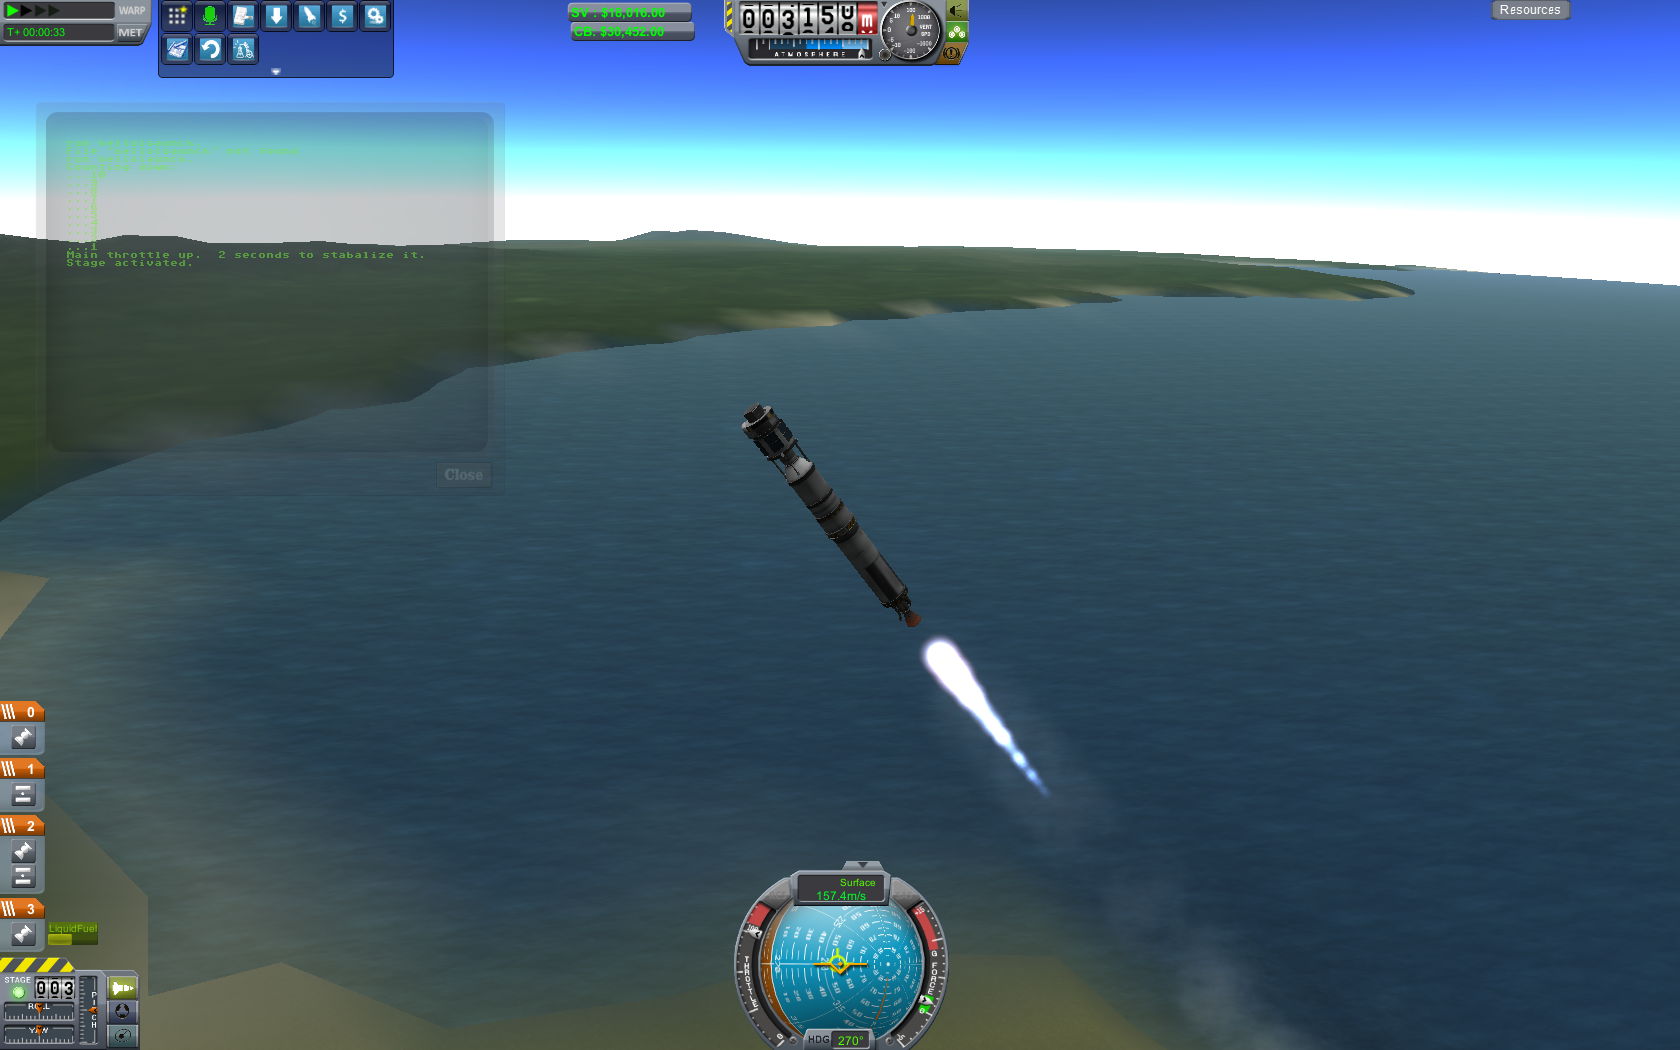
\includegraphics[width=3in]{example_2_2.png}
\end{center}

Hey! It does something now! It fires the first stage engine and launches!

But.. but wait... It doesn?t control the steering and it just lets it go where ever it will.

Most likely you had a crash with this script because it didn?t do anything to affect the steering at all, so it probably allowed the rocket to tilt over.

\paragraph{Step 4: Make the script actually control steering}
So to fix that problem, let?s add steering control to the script.

The easy way to control steering is to use the LOCK STEERING command.

Once you have mastered the basics of kOS, you should go and read the documentation on ship steering techniques, but that?s a more advanced topic for later.

The way to use the LOCK STEERING command is to set it to a thing called a Vector or a Direction. There are several Directions built-in to kOS, one of which is called ?UP?. ?UP? is a Direction that always aims directly toward the sky (the center of the blue part of the navball).

So to steer always UP, just do this:

\begin{lstlisting}[frame=single,language=XML]
LOCK STEERING TO UP.
\end{lstlisting} 

So if you just add this one line to your script, you?ll get something that should keep the craft aimed straight up and not let it tip over. Add the line just after the line that sets the THROTTLE, like so:

\begin{lstlisting}[frame=single,language=XML]
// My First Launcher.

PRINT "Counting down:".
FROM {local countdown is 10.} UNTIL countdown = 0 STEP {SET countdown to countdown - 1.} DO {
    PRINT "..." + countdown.
    WAIT 1. // pauses the script here for 1 second.
}
PRINT "Main throttle up.  2 seconds to stabalize it.".
LOCK THROTTLE TO 1.0.   // 1.0 is the max, 0.0 is idle.


LOCK STEERING TO UP.  // This is the new line to add


WAIT 2. // give throttle time to adjust.
UNTIL SHIP:MAXTHRUST > 0 {
    WAIT 0.5. // pause half a second between stage attempts.
    PRINT "Stage activated.".
    STAGE. // same as hitting the spacebar.
}
WAIT UNTIL SHIP:ALTITUDE > 70000. // pause here until ship is high up.

// NOTE that it is vital to not just let the script end right away
// here.  Once a kOS script just ends, it releases all the controls
// back to manual piloting so that you can fly the ship by hand again.
// If the pogram just ended here, then that would cause the throttle
// to turn back off again right away and nothing would happen.
\end{lstlisting} 

Again, copy this and run it, like before. If your craft crashed in the previous step, which it probably did, then revert to the VAB and re-launch it. NOTE: Due to a bug sometimes reverting just to the launchpad does not work well and you need to revert all the way back to the VAB.:

\begin{lstlisting}[frame=single,language=XML]
SWITCH TO 1. // should be the default already, but just in case.
COPY HELLOLAUNCH FROM 0.
RUN HELLOLAUNCH.
\end{lstlisting} 

\begin{center}
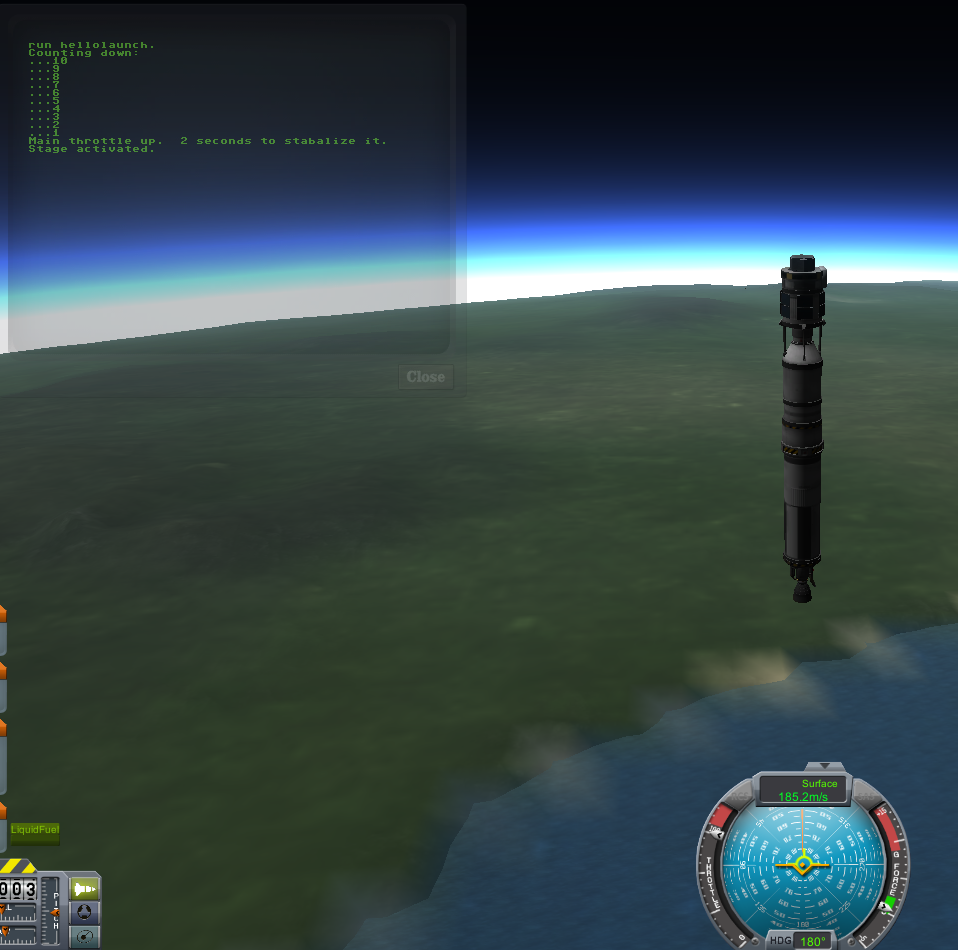
\includegraphics[width=3in]{example_2_3.png}
\end{center}

Now you should see the same thing as before, but now your craft will stay pointed up.

But wait - it only does the first stage and then it stops without doing the next stage? how do I fix that?

\paragraph{Step 5: Add staging logic}
The logic for how and when to stage can be an interesting and fun thing to write yourself. This example will keep it very simple, and this is the part where it?s important that you are using a vessel that only contains liquidfuel engines. If your vessel has some booster engines, then it would require a more sophisticated script to launch it correctly than this tutorial gives you.

To add the logic to check when to stage, we introduce a new concept called the WHEN trigger. To see full documentation on it when you finish the tutorial, look for it on the Flow Control page

The quick and dirty explanation is that a WHEN section is a short section of code that you set up to run LATER rather than right now. It creates a check in the background that will constantly look for some condition to occur, and when it happens, it interrupts whatever else the code is doing, and it will run the body of the WHEN code before continuing from where it left off in the main script.

There are some complex dangers with writing WHEN triggers that can cause KSP itself to hang or stutter if you are not careful, but explaining them is beyond the scope of this tutorial. But when you want to start using WHEN triggers yourself, you really should read the section on WHEN in the Flow Control page before you do so.

The WHEN trigger we are going to add to the launch script looks like this:

\begin{lstlisting}[frame=single,language=XML]
WHEN STAGE:LIQUIDFUEL < 0.001 THEN {
    PRINT "No liquidfuel.  Attempting to stage.".
    STAGE.
    PRESERVE.
}
\end{lstlisting} 

It says, ?Whenever the amount of liquid fuel in the current stage is so small it may as well be zero (< 0.001), then activate the next stage.? The PRESERVE keyword says, ?don?t stop checking this condition just because it?s been triggered once. It should still keep checking for it again in the future.? The check for < 0.001 is because sometimes KSP won?t quite burn the last drop of fuel in a stage. If this block of code is inserted into the script, then it will set up a constant background check that will always hit the next stage as soon as the current stage has no liquidfuel in it. UNLIKE with all the previous edits this tutorial has asked you to make to the script, this time you?re going to be asked to delete something and replace it. The new WHEN section above should actually REPLACE the existing ?UNTIL SHIP:MAXTHRUST > 0? loop that you had before.

Now your script should look like this:

\begin{lstlisting}[frame=single,language=XML]
// My First Launcher.

PRINT "Counting down:".
FROM {local countdown is 10.} UNTIL countdown = 0 STEP {SET countdown to countdown - 1.} DO {
    PRINT "..." + countdown.
    WAIT 1. // pauses the script here for 1 second.
}
PRINT "Main throttle up.  2 seconds to stabalize it.".
LOCK THROTTLE TO 1.0.   // 1.0 is the max, 0.0 is idle.
LOCK STEERING TO UP.
WAIT 2. // give throttle time to adjust.

// The section below replaces previous UNTIL loop:

WHEN STAGE:LIQUIDFUEL < 0.001 THEN {
    PRINT "No liquidfuel.  Attempting to stage.".
    STAGE.
    PRESERVE.
}
WAIT UNTIL SHIP:ALTITUDE > 70000. // pause here until ship is high up.

// NOTE that it is vital to not just let the script end right away
// here.  Once a kOS script just ends, it releases all the controls
// back to manual piloting so that you can fly the ship by hand again.
// If the pogram just ended here, then that would cause the throttle
// to turn back off again right away and nothing would happen.
\end{lstlisting} 
Again, relaunch the ship, copy the script as before, and run it again. This time you should see it activate your later upper stages correctly. (again, assuming you made the entire vessel with only liquidfuel engines.)

\begin{center}
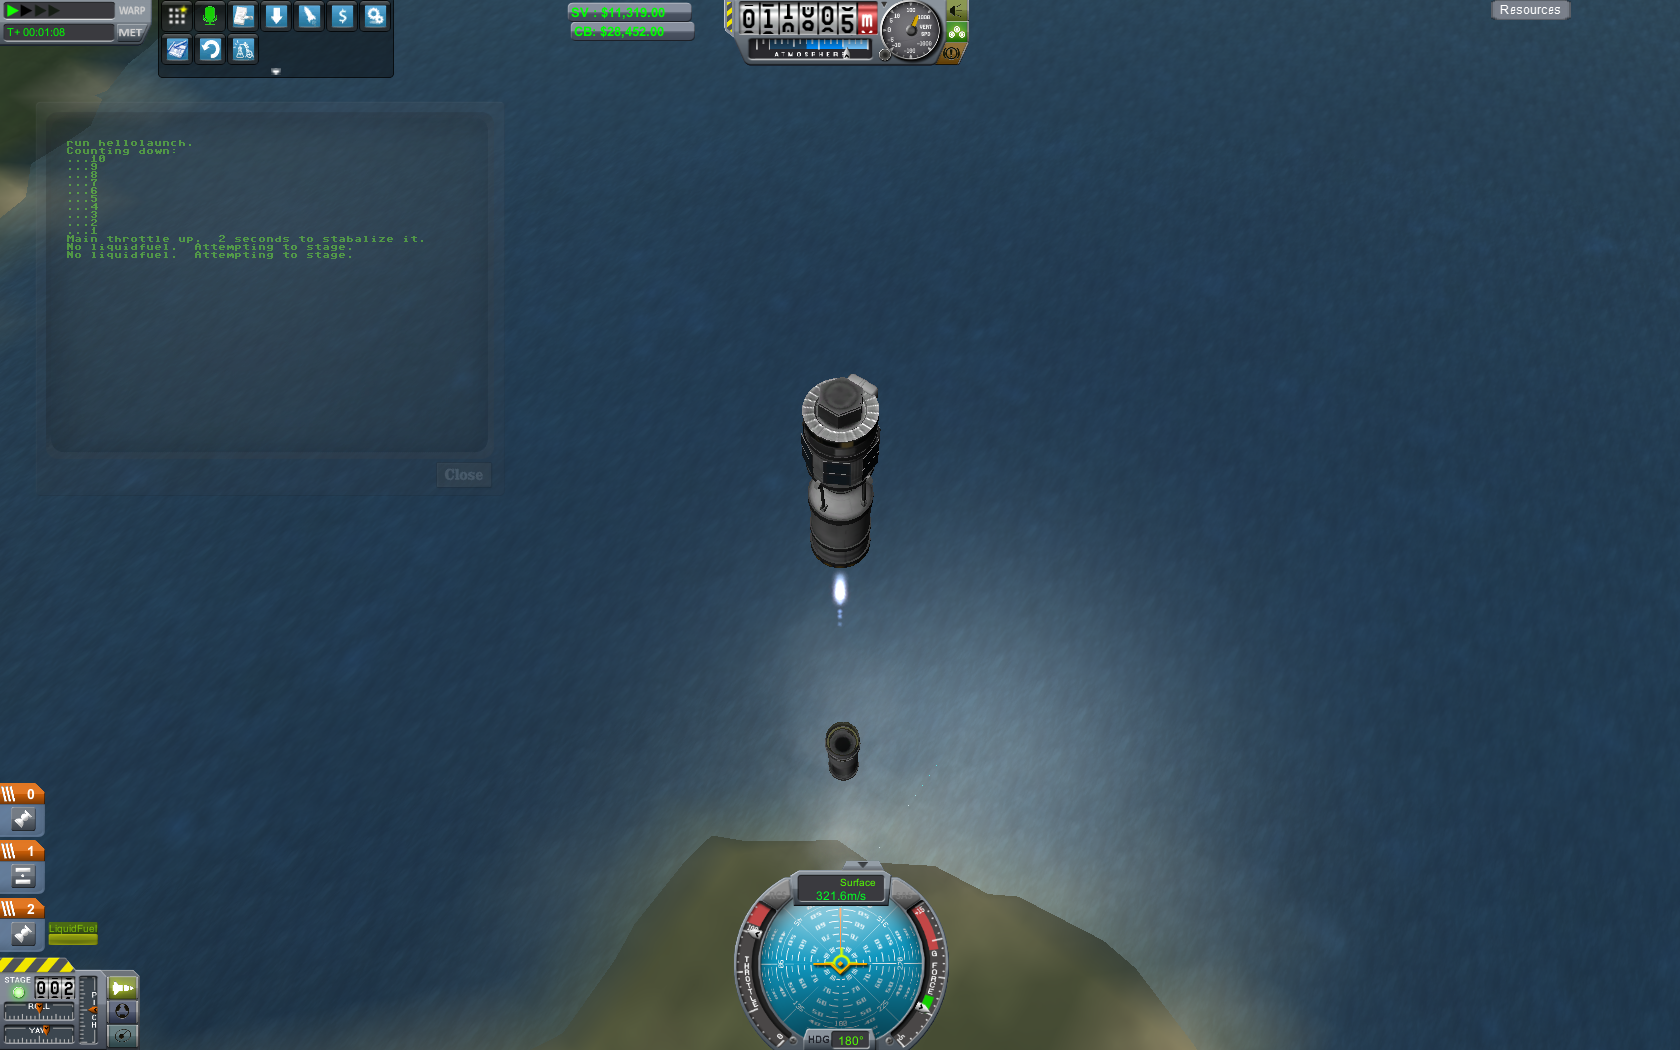
\includegraphics[width=3in]{example_2_4.png}
\end{center}

\paragraph{Step 6: Now to make it turn}
Okay that?s fine but it still just goes straight up! What about a gravity turn?

Well, a true and proper gravity turn is a very complex bit of math that is best left as an excercise for the reader, given that the goal of kOS is to let you write your OWN autopilot, not to write it for you. But to give some basic examples of commands, lets just make a crude gravity turn approximation that simply flies the ship like a lot of new KSP pilots learn to do it for the first time:

Fly straight up to 10000m.
Aim at 45 degrees down toward the east until 40000m.
Thrust horizontally east after that.
To make this work, we introduce a new way to make a Direction, called the HEADING function. Whenever you call the function HEADING(a,b), it makes a Direction oriented as follows on the navball:

Point at the compass heading A.
Pitch up a number of degrees from the horizon = to B.
So for example, HEADING(45,10) would aim northeast, 10 degrees above the horizon. Combining this with the WHEN command from before, we get this section:

\begin{lstlisting}[frame=single,language=XML]
WHEN SHIP:ALTITUDE > 10000 THEN {
    PRINT "Starting turn.  Aiming to 45 degree pitch.".
    LOCK STEERING TO HEADING(90,45). // east, 45 degrees pitch.
}
WHEN SHIP:ALTITUDE > 40000 THEN {
    PRINT "Starting flat part.  Aiming to horizon.".
    LOCK STEERING TO HEADING(90,0). // east, horizontal.
}
\end{lstlisting} 

Note that these lack the command PRESERVE like the previous WHEN example had. This is because we want these to trigger just once and then never again. There?s no point in constantly telling kOS to reset the steering to the same thing over and over as the script runs.

Now, if you insert this new section to the script, we have a nice nifty example of a start of a launching script. Note that it works even if you insert it at the top of the script, because it sets up the triggers to occur LATER when the condition becomes true. They don?t execute right away:

\begin{lstlisting}[frame=single,language=XML]
// My First Launcher.

WHEN SHIP:ALTITUDE > 10000 THEN {
    PRINT "Starting turn.  Aiming to 45 degree pitch.".
    LOCK STEERING TO HEADING(90,45). // east, 45 degrees pitch.
}
WHEN SHIP:ALTITUDE > 40000 THEN {
    PRINT "Starting flat part.  Aiming to horizon.".
    LOCK STEERING TO HEADING(90,0). // east, horizontal.
}
PRINT "Counting down:".
FROM {local countdown is 10.} UNTIL countdown = 0 STEP {SET countdown to countdown - 1.} DO {
    PRINT "..." + countdown.
    WAIT 1. // pauses the script here for 1 second.
}
PRINT "Main throttle up.  2 seconds to stabalize it.".
LOCK THROTTLE TO 1.0.   // 1.0 is the max, 0.0 is idle.
LOCK STEERING TO UP.
WAIT 2. // give throttle time to adjust.

// The section below replaces previous UNTIL loop:

WHEN STAGE:LIQUIDFUEL < 0.001 THEN {
    PRINT "No liquidfuel.  Attempting to stage.".
    STAGE.
    PRESERVE.
}
WAIT UNTIL SHIP:ALTITUDE > 70000. // pause here until ship is high up.

// NOTE that it is vital to not just let the script end right away
// here.  Once a kOS script just ends, it releases all the controls
// back to manual piloting so that you can fly the ship by hand again.
// If the program just ended here, then that would cause the throttle
// to turn back off again right away and nothing would happen.
\end{lstlisting} 

And here is it in action:

\begin{center}
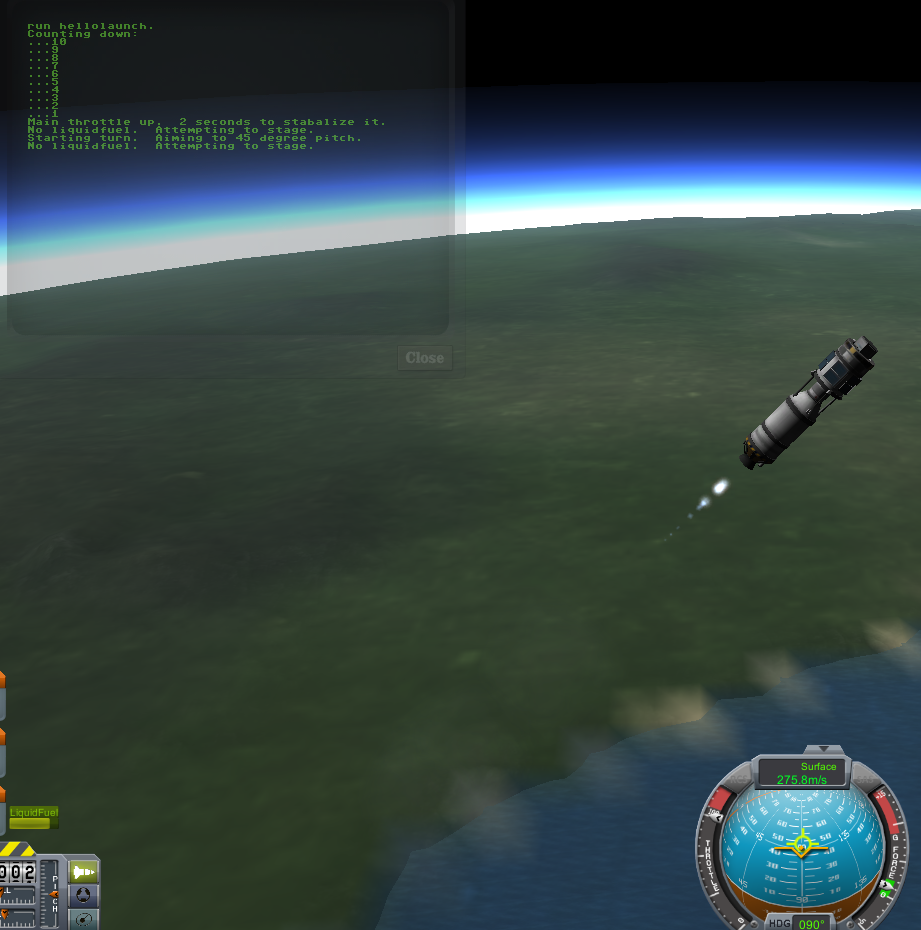
\includegraphics[width=3in]{example_2_5.png}
\end{center}

And toward the end:

\begin{center}
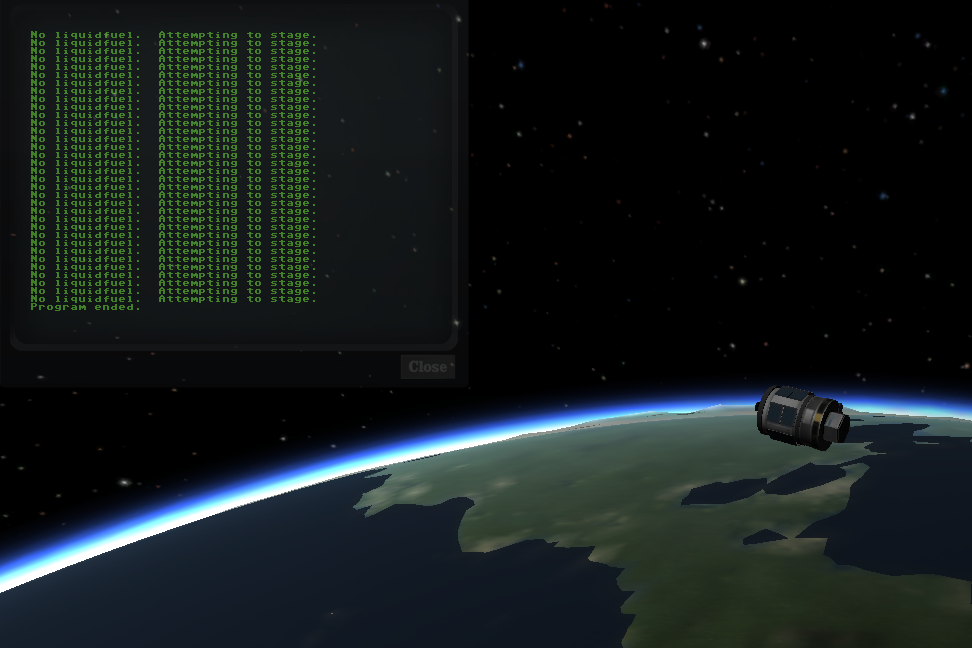
\includegraphics[width=3in]{example_2_6.png}
\end{center}

If we assume you made a vessel that has enough fuel and power to get up to orbit, this script should in principle work to get you to the point of leaving the atmosphere. It will probably still fall back down, because this script makes no attempt to ensure that the craft is going fast enough to maintain the orbit.

As you can probably see, it would still have a long way to go before it would become a really GOOD launching autopilot. Think about the following features you could add yourself as you become more familiar with kOS:

You could change the steering logic to make a more smooth gravity turn by constantly adjusting the pitch in the HEADING according to some math formula. The example shown here tends to create a ?too high? launch that?s a bit inefficient.
You could complete the launching script by making sure once the vessel breaks the atmosphere it actually makes a circular orbit rather than just stopping after 70000m and coasting.
This script just stupidly leaves the throttle at max the whole way. You could make it more sophisticated by adjusting the throttle as necessary to avoid too much wasted energy fighting air friction. (The way KSP?s stock areodynamic model works, the optimal speed is terminal velocity, by the way). This is partly addressed in the PID Loop Tutorial.
With more sophisticated staging checks, the script could be made to work with solid fuel engines as well.
With even more sophisticated checks, the script could be made to work with fancy staging methods like asaparagus.
Using the PRINT AT command, you can make fancier status readouts in the termainl window as the script runs.
	\section{Design Patterns and Considerations with kOS} %%%%% SECTION %%%%%
	
There are many ways one can write a control program for a given scenario. The goal of this section is to help a novice kOS programmer, after having finished the Quick Start Tutorial, to develop a sense of elegance and capability when writing his or her own kOS scripts. All of the examples in this tutorial may be tested by the reader using a rocket design similar to the following. Notice it carries an accelerometer and the negative gravioli detector which are used in the second section. Don?t forget the kOS module as well!

\begin{center}
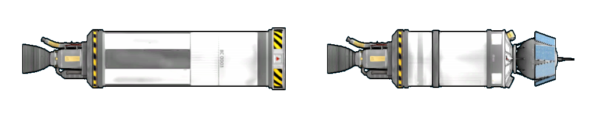
\includegraphics[width=3in]{designpatterns_rocket.png}
\end{center}

\subsection{The Major Design Patterns of kOS Control Programs}
The design of a program is usually determined by the flow-control statements used. I.e., the WHEN/THEN, ON, WAIT, UNTIL, IF and FOR constructs. Here is a list of the major styles of control programs that can be written in kOS:

Sequential
Loops with Condition Checking
Loops with Triggers
Of course, one style does not fit all scenarios and the programmer will typically want to use a combination of these all at once. Also, there may be other design patterns not listed here which can be perfectly valid, but this is a start.

\paragraph{1. Sequential Programs}
These are programs that rely almost exclusively on WAIT UNTIL statements to go from one phase to the next.

\begin{lstlisting}[frame=single,language=XML]
LOCK STEERING TO HEADING(0,90).
LOCK THROTTLE TO 1.
STAGE.
WAIT UNTIL SHIP:ALTITUDE > 10000.
LOCK STEERING TO HEADING(0,90) + R(0,-45,0).
WAIT UNTIL STAGE:LIQUIDFUEL < 0.1.
STAGE.
WAIT UNTIL SHIP:ALTITUDE > 20000.
LOCK THROTTLE TO 0.
WAIT UNTIL FALSE. // CTRL+C to break out
\end{lstlisting} 

This example will take a two stage rocket up to 20km. The immediate thing to notice is that the programmer must have known that the first stage would cutoff between 10km and 20km. This is fine for a specific rocket but not too general and could end in disaster if the first stage cutoff occurs at say 5km. Certainly, one can write a program using this technique to take a specific rocket, put it into orbit and even perform a lot of fancy maneuvers, but adapting the code to different rockets may get complicated quickly.

\paragraph{2. Loops with Condition Checking}
Here, we introduce IF/ELSE logic into UNTIL loops:

\begin{lstlisting}[frame=single,language=XML]
LOCK STEERING TO R(0,0,-90) + HEADING(90,90).
LOCK THROTTLE TO 1.
STAGE.
UNTIL SHIP:ALTITUDE > 20000 {
    IF SHIP:ALTITUDE > 10000 {
        LOCK STEERING TO R(0,0,-90) + HEADING(90,45).
    }
    IF STAGE:LIQUIDFUEL < 0.1 {
        STAGE.
    }
}
LOCK THROTTLE TO 0.
WAIT UNTIL FALSE.
\end{lstlisting} 

This does the same thing as the previous example, but now it?s checking for a staging condition from the launch pad all the way to 20km. More than that, it will stage as many times as needed.

One can imagine that these types of UNTIL loops can become very complex with many layers of IF/ELSE blocks. Once this happens it is usually good to reduce the frequency of the loop by adding a WAIT statement at the end of the loop. This wait could be anywhere from 0.001 (every physics tick), to 60 (every minute) or even longer for inter-planetary transfers if desired.

3. Loops with Triggers
In the above example, once the rocket reaches 10km, the steering is constantly being re-locked to HEADING(90,45). This works, but it only needs to be locked once. A possible improvement is to set up a trigger using a WHEN/THEN statement:

\begin{lstlisting}[frame=single,language=XML]
LOCK STEERING TO R(0,0,-90) + HEADING(90,90).
LOCK THROTTLE TO 1.
STAGE.
WHEN SHIP:ALTITUDE > 10000 THEN {
    LOCK STEERING TO R(0,0,-90) + HEADING(90,45).
}
UNTIL SHIP:ALTITUDE > 20000 {
    IF STAGE:LIQUIDFUEL < 0.1 {
        STAGE.
    }
}
LOCK THROTTLE TO 0.
WAIT UNTIL FALSE.
\end{lstlisting} 

Now, when the rocket reaches 10km, the steering is set once and the trigger is removed from the active list of triggers. The staging condition can also be promoted to a trigger, keeping the trigger active after every stage using the PRESERVE keyword:

\begin{lstlisting}[frame=single,language=XML]
WHEN STAGE:LIQUIDFUEL < 0.1 THEN {
    STAGE.
    PRESERVE.
}
LOCK STEERING TO R(0,0,-90) + HEADING(90,90).
LOCK THROTTLE TO 1.
STAGE.
WHEN SHIP:ALTITUDE > 10000 THEN {
    LOCK STEERING TO R(0,0,-90) + HEADING(90,45).
}
WAIT UNTIL SHIP:ALTITUDE > 20000.
LOCK THROTTLE TO 0.
WAIT UNTIL FALSE.
\end{lstlisting} 

Notice that the UNTIL loop was changed to a WAIT UNTIL statement since the program is small and all the logic of the triggers can be handled in a reasonable amount of time - there will be more on this topic later.

\paragraph{Bringing It All Together}
Typically, the programmer will find all of these constructs are useful at the same time and kOS scripts will naturally contain some sequential parts in combination with long-term and short-term triggers which can modify states in complex loops of varying frequency. If you didn?t follow that bit of gobbledygook, don?t worry. The next section will discuss a few recommendations for beginning kOS programmers to follow when setting up any program.

\subsection{General Guidelines for kOS Scripts}
This section discusses two general guidelines to follow when starting out with more complicated kOS scripts. These are not meant to be absolute and there will certainly be cases when they can be stretched, though one should never totally ignore them.

\paragraph{1. Minimize Time Spent in WHEN/THEN Blocks}
Remember that WAIT statements are ignored when inside WHEN/THEN blocks. It is OK to loop over small lists (engines for example), but don?t let it get out of hand. The WHEN/THEN construct was designed to accommodate quick bits of code. Consider this bit of (non-working) code which tries to adjust the throttle based on the g-force as measured by a combination of the accelerometer and the negative gravioli detector:

\begin{lstlisting}[frame=single,language=XML]
SET thrott TO 1.
LOCK THROTTLE TO thrott.
LOCK STEERING TO R(0,0,-90) + HEADING(90,90).
STAGE.
WHEN SHIP:ALTITUDE > 1000 THEN {
    SET g TO KERBIN:MU / KERBIN:RADIUS^2.
    LOCK accvec TO SHIP:SENSORS:ACC - SHIP:SENSORS:GRAV.
    LOCK gforce TO accvec:MAG / g.
    LOCK dthrott TO 0.05 * (1.2 - gforce).

    UNTIL SHIP:ALTITUDE > 40000 {
        WHEN STAGE:LIQUIDFUEL < 0.1 THEN {
            STAGE.
            PRESERVE.
        }
        SET thrott to thrott + dthrott.
        WAIT 0.1.
    }
}
\end{lstlisting} 

This looks reasonable. The throttle is set to maximum until 1km is reached at which point the throttle is adjusted every 0.1 seconds. If the gforce is off from the value of 1.2, then the throttle is either increased or decreased by a small amount. Running this on a test rocket merely produce the message ?Program ended.?

Understanding why this does not work is important. Everything in a WHEN/THEN block is expected to complete in the current physics tick, but here we have a loop that is supposed to last until the ship reaches 40km. This example can be reworked by separating the triggers from the loop. The staging trigger was separated from the UNTIL loop as well - not strictly necessary, but recommended form:

\begin{lstlisting}[frame=single,language=XML]
WHEN STAGE:LIQUIDFUEL < 0.1 THEN {
    STAGE.
    PRESERVE.
}
SET thrott TO 1.
SET dthrott TO 0.
LOCK THROTTLE TO thrott.
LOCK STEERING TO R(0,0,-90) + HEADING(90,90).
STAGE.
WHEN SHIP:ALTITUDE > 1000 THEN {
    SET g TO KERBIN:MU / KERBIN:RADIUS^2.
    LOCK accvec TO SHIP:SENSORS:ACC - SHIP:SENSORS:GRAV.
    LOCK gforce TO accvec:MAG / g.
    LOCK dthrott TO 0.05 * (1.2 - gforce).
}
UNTIL SHIP:ALTITUDE > 40000 {
    SET thrott to thrott + dthrott.
    WAIT 0.1.
}
\end{lstlisting} 

Now this program should work. The variable dthrott had to be set to 0 in the beginning so that the throttle is kept at maximum until 1km, the UNTIL loop operates every 0.1 seconds, and the WHEN/THEN triggers are run only once when the condition is met. The take-away from this example is to keep WHEN/THEN blocks separate from UNTIL loops. Specifically, never put an UNTIL loop inside a WHEN/THEN block and it should be extremely rare to put a WHEN/THEN statement inside an UNTIL loop.

Finally, as a bit of foreshadowing, this bit of code is actually a ?proportional feedback loop.? From an altitude of 1km up to 40km, the total g-force exerted on the ship is kept near 1.2 by constantly adjusting the throttle. The value of 1.2 is called the ?setpoint,? the measured g-force is called the ?process variable,? and the mystical 0.05 is called the ?proportional gain.? Please take a look at the PID Loop Tutorial which takes this script as a starting point and develops a full PID-loop in kOS.

\paragraph{2. Minimize Trigger Conditions}
There is a lot of power in developing multi-level LOCK variables in combination with WHEN/THEN triggers. However, it can be easy to hit kOS?s hard limit in the number of operations allowed for trigger checking. This will happen when several WHEN/THEN triggers are dependent on the same complex LOCK variable. This results in the LOCK variable being calculated multiple times every update. If the LOCK is deep enough, the calculations become too expensive to do and kOS stops executing and complains.

With this in mind, consider an extension of the example script in the previous section. This time, the g-force setpoint changes as the rocket climbs through 10km, 20km and 30km:

\begin{lstlisting}[frame=single,language=XML]
WHEN STAGE:LIQUIDFUEL < 0.1 THEN {
    STAGE.
    PRESERVE.
}
SET thrott TO 1.
SET dthrott TO 0.
LOCK THROTTLE TO thrott.
LOCK STEERING TO R(0,0,-90) + HEADING(90,90).
STAGE.
WHEN SHIP:ALTITUDE > 1000 THEN {
    SET g TO KERBIN:MU / KERBIN:RADIUS^2.
    LOCK accvec TO SHIP:SENSORS:ACC - SHIP:SENSORS:GRAV.
    LOCK gforce TO accvec:MAG / g.
    LOCK dthrott TO 0.05 * (1.2 - gforce).
}
WHEN SHIP:ALTITUDE > 10000 THEN {
    LOCK dthrott TO 0.05 * (2.0 - gforce).
}
WHEN SHIP:ALTITUDE > 20000 THEN {
    LOCK dthrott TO 0.05 * (4.0 - gforce).
}
WHEN SHIP:ALTITUDE > 30000 THEN {
    LOCK dthrott TO 0.05 * (5.0 - gforce).
}
UNTIL SHIP:ALTITUDE > 40000 {
    SET thrott to thrott + dthrott.
    WAIT 0.1.
}
\end{lstlisting} 

This example does what is expected of it without problems. But the ship?s altitude is being checked at least five times for every update, including the UNTIL loop check. Certaintly, the kOS CPU can keep up with this, however, one can imagine a whole series of WHEN/THEN statements which make use of complicated calculations based on atmospheric data or orbital mechanics. One way to minimize the trigger condition checking is to take strictly-sequential triggers and nest them:

\begin{lstlisting}[frame=single,language=XML]
WHEN STAGE:LIQUIDFUEL < 0.1 THEN {
    STAGE.
    PRESERVE.
}
SET thrott TO 1.
SET dthrott TO 0.
LOCK THROTTLE TO thrott.
LOCK STEERING TO R(0,0,-90) + HEADING(90,90).
STAGE.
WHEN SHIP:ALTITUDE > 1000 THEN {
    SET g TO KERBIN:MU / KERBIN:RADIUS^2.
    LOCK accvec TO SHIP:SENSORS:ACC - SHIP:SENSORS:GRAV.
    LOCK gforce TO accvec:MAG / g.
    LOCK dthrott TO 0.05 * (1.2 - gforce).

    WHEN SHIP:ALTITUDE > 10000 THEN {
        LOCK dthrott TO 0.05 * (2.0 - gforce).

        WHEN SHIP:ALTITUDE > 20000 THEN {
            LOCK dthrott TO 0.05 * (4.0 - gforce).

            WHEN SHIP:ALTITUDE > 30000 THEN {
                LOCK dthrott TO 0.05 * (5.0 - gforce).
            }
        }
    }
}
UNTIL SHIP:ALTITUDE > 40000 {
    SET thrott to thrott + dthrott.
    WAIT 0.1.
}
\end{lstlisting} 

Now this is quite elegant! The number of triggers have been reduced to two per update for the entire running of this script. The trigger at 1km sets up the next trigger which will happen at 10km which sets up then next at 20km and so on. This can save a lot of processing time for triggers that will happen sequentially. As a general rule, one should try to nest WHEN/THEN statements whenever possible. Again, both examples above will work, but when scripts start to have deep and complicated triggers, this nested construct can save it from the dreaded kOS trigger limit.

	\section{PID Loops in k-OS}%%%%% NEXT SECTION %%%%%
	
This tutorial covers how one can implement a PID loop using kOS. A P-loop, or ?proportional feedback loop? was already introduced in the second section of the Design Patterns Tutorial, and that will serve as our starting point. After some code rearrangement, the integral and derivative terms will be added and discussed in turn. Next, a couple extra features will be added to the full PID-loop. Lastly, we?ll show a case-study in tuning a full PID loop using the Ziegler-Nichols method. We?ll use the LOG method to dump telemetry from KSP into a file and our favorite graphing software to visualize the data.

The code examples in this tutorial can be tested with a similar rocket design as shown. Do not forget the accelerometer, gravioli detector or the kOS CPU module. The engine is purposefully overpowered to demonstrate the feedback in action.

\begin{center}
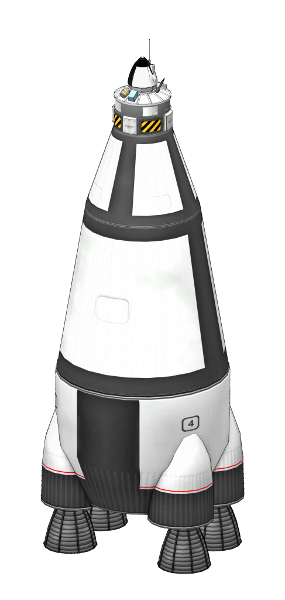
\includegraphics[height=4in]{pidtune_rocket_design_maxtwr8.png}
\end{center}

Those fuel-tank adapters are from the Modular Rocket Systems (MRS) addon, but stock tanks will work just fine. The design goal of this rocket is to have a TWR of 8 on the launchpad and enough fuel to make it past 30km when throttled for optimal atmospheric efficiency.

\paragraph{Proportional Feedback Loop (P-loop)}
The example code from the Design Patterns Tutorial, with some slight modifications looks like the following:

\begin{lstlisting}[frame=single,language=XML]
// staging, throttle, steering, go
WHEN STAGE:LIQUIDFUEL < 0.1 THEN {
    STAGE.
    PRESERVE.
}
LOCK THROTTLE TO 1.
LOCK STEERING TO R(0,0,-90) + HEADING(90,90).
STAGE.
WAIT UNTIL SHIP:ALTITUDE > 1000.

// P-loop setup
SET g TO KERBIN:MU / KERBIN:RADIUS^2.
LOCK accvec TO SHIP:SENSORS:ACC - SHIP:SENSORS:GRAV.
LOCK gforce TO accvec:MAG / g.
LOCK dthrott TO 0.05 * (1.2 - gforce).

SET thrott TO 1.
LOCK THROTTLE to thrott.

UNTIL SHIP:ALTITUDE > 40000 {
    SET thrott to thrott + dthrott.
    WAIT 0.1.
}
\end{lstlisting} 

The first several lines sets up a simple staging condition, puts the throttle to maximum, steers the rocket straight up and launches. The rocket is assumed to use only liquid fuel engines. After the rocket hits 1km, the script sets up the LOCK used in the P-loop which is updated every 0.1 seconds in the UNTIL loop. The use of LOCK variables makes this code fairly clean. When the script comes up to the first line in the UNTIL loop, i.e. ?SET thrott TO thrott + dthrott.?, the variable dthrott is evaluated which causes the LOCK on gforce to be evaluated which in-turn causes accvec to be evaluated.

The input to this feedback loop is the acceleration experienced by the ship (gforce) in terms of Kerbin?s gravitational acceleration at sea level (g). The variable accvec is the total acceleration vector and is obtained by the accelerometer and gravioli detectors, both of which must be on the ship for this to work. The variable dthrott is the change in throttle that should be applied in a single iteration of the feedback loop.

In terms of a PID loop, the factor 1.2 is called the setpoint, gforce is the process variable and 0.05 is called the proportional gain. The setpoint and gain factors can be promoted to their own variables with names. Also, the code up to and including the ?WAIT UNTIL SHIP:ALTITUDE > 1000.? will be implied for the next few examples of code:

\begin{lstlisting}[frame=single,language=XML]
// P-loop
SET g TO KERBIN:MU / KERBIN:RADIUS^2.
LOCK accvec TO SHIP:SENSORS:ACC - SHIP:SENSORS:GRAV.
LOCK gforce TO accvec:MAG / g.

SET gforce_setpoint TO 1.2.
SET Kp TO 0.05.
LOCK dthrott TO Kp * (gforce_setpoint - gforce).

SET thrott TO 1.
LOCK THROTTLE to thrott.

UNTIL SHIP:ALTITUDE > 40000 {
    SET thrott to thrott + dthrott.
    WAIT 0.1.
}
\end{lstlisting} 

This is not a big change, but it will set us up to include the integral and derivative terms in the next section.

\paragraph{Proportional-Integral Feedback Loop (PI-loop)}
Adding the integral term requires us to keep track of time. This is done by introducing a variable (t0) to store the time of the last iteration. Now, the throttle is changed only on iterations where some time has elapsed so the WAIT time in the UNTIL can be brought to 0.001. The offset of the gforce has been set to the variable P, and the integral gain to Ki.

\begin{lstlisting}[frame=single,language=XML]
// PI-loop
SET g TO KERBIN:MU / KERBIN:RADIUS^2.
LOCK accvec TO SHIP:SENSORS:ACC - SHIP:SENSORS:GRAV.
LOCK gforce TO accvec:MAG / g.

SET gforce_setpoint TO 1.2.

LOCK P TO gforce_setpoint - gforce.
SET I TO 0.

SET Kp TO 0.01.
SET Ki TO 0.006.

LOCK dthrott TO Kp * P + Ki * I.

SET thrott TO 1.
LOCK THROTTLE to thrott.

SET t0 TO TIME:SECONDS.
UNTIL SHIP:ALTITUDE > 40000 {
    SET dt TO TIME:SECONDS - t0.
    IF dt > 0 {
        SET I TO I + P * dt.
        SET thrott to thrott + dthrott.
        SET t0 TO TIME:SECONDS.
    }
    WAIT 0.001.
}
\end{lstlisting} 

Adding the integral term has the general effect of stabilizing the feedback loop, making it less prone to oscillating due to rapid changes in the process variable (gforce, in this case). This is usually at the expense of a longer settling time.

\paragraph{Proportional-Integral-Derivative Feedback Loop (PID-loop)}
Incorporating the derivative term (D) and derivative gain (Kd) requires an additional variable (P0) to keep track of the previous value of the proportional term (P).

\begin{lstlisting}[frame=single,language=XML]
// PID-loop
SET g TO KERBIN:MU / KERBIN:RADIUS^2.
LOCK accvec TO SHIP:SENSORS:ACC - SHIP:SENSORS:GRAV.
LOCK gforce TO accvec:MAG / g.

SET gforce_setpoint TO 1.2.

LOCK P TO gforce_setpoint - gforce.
SET I TO 0.
SET D TO 0.
SET P0 TO P.

SET Kp TO 0.01.
SET Ki TO 0.006.
SET Kd TO 0.006.

LOCK dthrott TO Kp * P + Ki * I + Kd * D.

SET thrott TO 1.
LOCK THROTTLE to thrott.

SET t0 TO TIME:SECONDS.
UNTIL SHIP:ALTITUDE > 40000 {
    SET dt TO TIME:SECONDS - t0.
    IF dt > 0 {
        SET I TO I + P * dt.
        SET D TO (P - P0) / dt.
        SET thrott to thrott + dthrott.
        SET P0 TO P.
        SET t0 TO TIME:SECONDS.
    }
    WAIT 0.001.
}
\end{lstlisting} 

When tuned properly, the derivative term will cause the PID-loop to act quickly without causing problematic oscillations. Later in this tutorial, we will cover a way to tune a PID-loop using only the proportional term called the Zieger-Nichols method.

\paragraph{Final Touches}
There are a few modifications that can make PID loops very robust. The following code example adds three range limits:

bounds on the Integral term which addresses possible integral windup
bounds on the throttle since it must stay in the range 0 to 1
a deadband to avoid changing the throttle due to small fluctuations
Of course, KSP is a simulator and small fluctuations are not observed in this particular loop. Indeed, the P-loop is sufficient in this example, but all these features are included here for illustration purposes and they could become useful for unstable aircraft or untested scenarios.

\begin{lstlisting}[frame=single,language=XML]
// PID-loop
SET g TO KERBIN:MU / KERBIN:RADIUS^2.
LOCK accvec TO SHIP:SENSORS:ACC - SHIP:SENSORS:GRAV.
LOCK gforce TO accvec:MAG / g.

SET gforce_setpoint TO 1.2.

LOCK P TO gforce_setpoint - gforce.
SET I TO 0.
SET D TO 0.
SET P0 TO P.

LOCK in_deadband TO ABS(P) < 0.01.

SET Kp TO 0.01.
SET Ki TO 0.006.
SET Kd TO 0.006.

LOCK dthrott TO Kp * P + Ki * I + Kd * D.

SET thrott TO 1.
LOCK THROTTLE to thrott.

SET t0 TO TIME:SECONDS.
UNTIL SHIP:ALTITUDE > 40000 {
    SET dt TO TIME:SECONDS - t0.
    IF dt > 0 {
        IF NOT in_deadband {
            SET I TO I + P * dt.
            SET D TO (P - P0) / dt.

            // If Ki is non-zero, then limit Ki*I to [-1,1]
            IF Ki > 0 {
                SET I TO MIN(1.0/Ki, MAX(-1.0/Ki, I)).
            }

            // set throttle but keep in range [0,1]
            SET thrott to MIN(1, MAX(0, thrott + dthrott)).

            SET P0 TO P.
            SET t0 TO TIME:SECONDS.
        }
    }
    WAIT 0.001.
}
\end{lstlisting} 

\paragraph{Tuning a PID-loop}
We are going to start with the same rocket design we have been using so far and actually tune the PID-loop using the Ziegler-Nichols method. This is where we turn off the integral and derivative terms in the loop and bring the proportional gain (Kp) up from zero to the point where the loop causes a steady oscillation with a measured period (Tu). At this point, the proportional gain is called the ?ultimate gain? (Ku) and the actual gains (Kp, Ki and Kd) are set according to this table taken from wikipedia:

Control Type	Kp	Ki	Kd
P	0.5 Ku	 	 
PI	0.45 Ku	1.2 Kp / Tu	 
PD	0.8 Ku	 	Kp Tu / 8
classic PID	0.6 Ku	2 Kp / Tu	Kp Tu / 8
Pessen Integral Rule	0.7 Ku	0.4 Kp / Tu	0.15 Kp Tu
some overshoot	0.33 Ku	2 Kp / Tu	Kp Tu / 3
no overshoot	0.2 Ku	2 Kp / Tu	Kp Tu / 3

An immediate problem to overcome with this method is that it assumes a steady state can be achieved. With rockets, there is never a steady state: fuel is being consumed, altitude and therefore gravity and atmosphere is changing, staging can cause major upsets in the feedback loop. So, this tuning method will be some approximation which should come as no surprise since it will come from experimental observation. All we need is enough of a steady state that we can measure the oscillations - both the change in amplitude and the period.

The script we?ll use to tune the highly overpowered rocket shown will launch the rocket straight up (using SAS) and will log data to an output file until it reaches 30km at which point the log file will be copied to the archive and the program will terminate. Also, this time the feedback loop will be based on the more realistic ?atmospheric efficiency.? The log file will contain three columns: time since launch, offset of atmospheric efficiency from the ideal (in this case, 1.0) and the ship?s maximum thrust. The maximum thrust will increase monotonically with time (this rocket has only one stage) and we?ll use both as the x-axis when plotting the offset on the y-axis.

\begin{lstlisting}[frame=single,language=XML]
DECLARE PARAMETER Kp.

LOCK g TO SHIP:BODY:MU / (SHIP:BODY:RADIUS + SHIP:ALTITUDE)^2.
LOCK maxtwr TO SHIP:MAXTHRUST / (g * SHIP:MASS).

// feedback based on atmospheric efficiency
LOCK surfspeed TO SHIP:VELOCITY:SURFACE:MAG.
LOCK atmoeff TO surfspeed / SHIP:TERMVELOCITY.
LOCK P TO 1.0 - atmoeff.

SET t0 TO TIME:SECONDS.
LOCK dthrott TO Kp*P.
SET start_time TO t0.

LOG "# Throttle PID Tuning" TO throttle_log.
LOG "# Kp: " + Kp TO throttle_log.
LOG "# t P maxtwr" TO throttle_log.

LOCK logline TO (TIME:SECONDS - start_time)
        + " " + P
        + " " + maxtwr.

SET thrott TO 1.
LOCK THROTTLE TO thrott.
SAS ON.
STAGE.
WAIT 3.

UNTIL SHIP:ALTITUDE > 30000 {
    SET dt TO TIME:SECONDS - t0.
    IF dt > 0 {
        SET thrott TO MIN(1,MAX(0,thrott + dthrott)).
        SET t0 TO TIME:SECONDS.
        LOG logline TO throttle_log.
    }
    WAIT 0.001.
}
COPY throttle_log TO 0.
\end{lstlisting} 

Give this script a short name, something like ?tune.txt? so that running is simple:

\begin{lstlisting}[frame=single,language=XML]
copy tune from 0.
run tune(0.5).
\end{lstlisting} 

After every launch completes, you?ll have to go into the archive directory and rename the output log file. Something like $?throttle_log.txt? ?> ?throttle.01.log? will help if you increment the index number each time. To analyze the data, plot the offset (P) as a function of time (t). Here, we show the results for three values of Kp: 0.002, 0.016 and 0.160, including the maximum TWR when Kp = 0.002 as the top x-axis. The maximum TWR dependence on time is different for the three values of Kp, but not by a lot.
$
\begin{center}
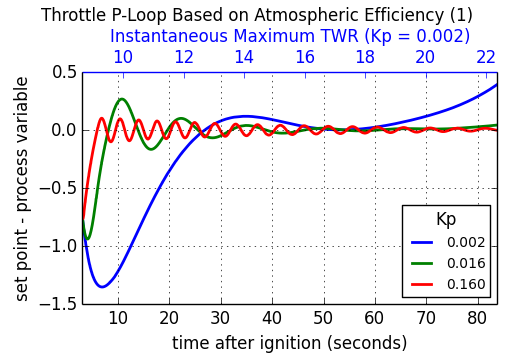
\includegraphics[width=3in]{pidtune1.png}
\end{center}

The value of 0.002 is obviously too low. The settling time is well over 20 seconds and the loop can?t keep up with the increase in terminal velocity at the higher altitudes reached after one minute. When Kp = 0.016, the behavior is far more well behaved, and though some oscillation exists, it?s damped and slow with a period of about 10 seconds. At Kp = 0.160, the oscillations are prominent and we can start to measure the change in amplitude along with the period of the oscillations. This plot shows the data for Kp = 0.160 from 20 to 40 seconds after ignition. The peaks are found and are fit to a line.

\begin{center}
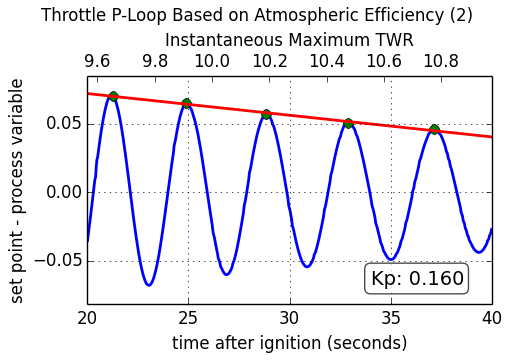
\includegraphics[width=3in]{pidtune2.png}
\end{center}

This is done for each value of Kp and the slopes of the fitted lines are plotted as a function of Kp in the following plot:

\begin{center}
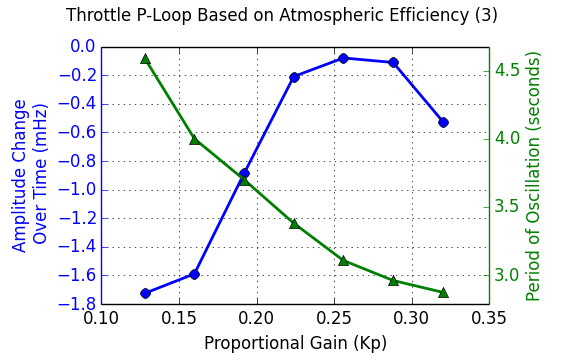
\includegraphics[width=3in]{pidtune3.png}
\end{center}

The period of oscillation was averaged over the interval and plotted on top of the amplitude change over time. Notice the turn over that occurs when Kp reaches approximately 0.26. This will mark the ?ultimate gain? and 3.1 seconds will be used as the associated period of oscillation. It is left as an exercise for the reader to implement a full PID-loop using the classic PID values (see table above): Kp = 0.156, Ki = 0.101, Kd = 0.060, producing this behavior:

\begin{center}
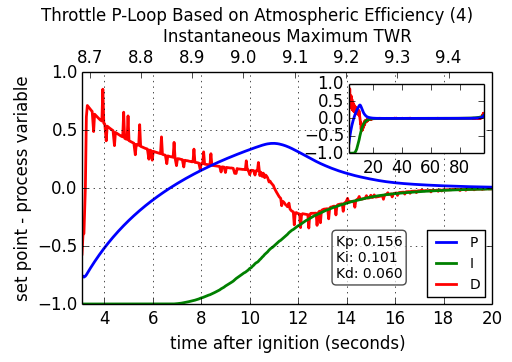
\includegraphics[width=3in]{pidtune4.png}
\end{center}

As soon as the PID-loop was activated at 3 seconds after ignition, the throttle was cut. At approximately 7 seconds, the atmospheric efficiency dropped below 100\% and the integral term started to climb back to zero. At 11 seconds, the engine was reignited and the feedback loop settled after about 20 seconds. The inset plot has the same axes as the parent and shows the long-term stability of the final PID-loop.

Final Thoughts
The classic PID values used above are fairly aggressive and there is some overshoot at the beginning. This can be dealt with in many ways and is discussed on the wikipedia page about PID controllers. For example, one might consider trying to implement a switch to a PD-loop when the integral term hits some limit, switching back once P crosses zero. The PID behavior should look like the following:

\begin{center}
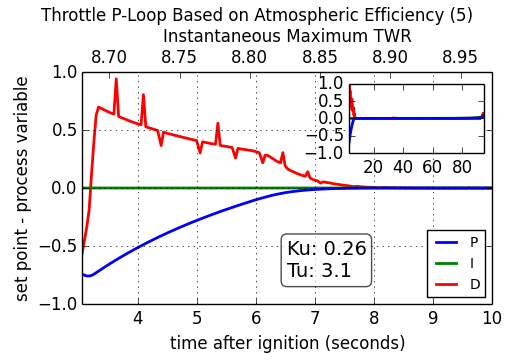
\includegraphics[width=3in]{pidtune5.png}
\end{center}

Finally, Controlling the throttle of a rocket is perhaps the easiest thing to implement as a PID loop in KSP using kOS. The steering was largely ignored and the orientation was always up. When writing an autopilot for horizontal atmospheric flight, one will have to deal with the direction the ship is traveling using SHIP:HEADING as well as it?s orientation with SHIP:FACING. Additionally, there are the SHIP:ROTATION and SHIP:TRANSLATION vectors which can tell you the rate of change of the ship?s facing and heading respectively. The controls in this case are six-dimensional using SHIP:CONTROL with YAW, PITCH, ROLL, FORE, STARBOARD, TOP and MAINTHROTTLE.

The PID gain parameters are dependent on the characteristics of the ship being controlled. The size, shape, turning capability and maximum TWR should be considered when tuning a PID loop. Turning RCS on can also have an effect and you might consider changing the PID loop?s gain parameters every time to switch them on or off.
	\section{Execute Node Script}
\part{General Code}
	\section{Bound Variables}
	\section{CPU Vessel (SHIP)}
	\section{CPU Hardware}
	\section{Launcher Panel}
	\section{Telnet Server}
	\section{Files and Volumes}
	\section{Machine Code}
	\section{Name Tags}
	\section{Parts and PartModules}
	\section{Respecting Career Limits}
\include{Lanuage}
\part{Mathematics}
	\section{Fundamental Constants}
	\section{Mathematical Functions}
	\section{Vectors}
	\section{Directions}
	\section{Geographic Coordinates}
	\section{Reference Frames}
\part{Commands}
	\section{Flight Control}
		\subsection{Cooked Control}
		\subsection{Raw Control}
		\subsection{Pilot Input}
		\subsection{Ship Systems}
		\subsection{Time Warping}
	\section{Prediction}
	\section{Listing Data}
	\section{Parts Information}
	\section{File I/O}
	\section{Termianl and GUI}
	\section{Resource Transfer}
\part{Structures}
	\section{Orbits}
		\subsection{Orbit}
		\subsection{Orbitable (Vessels and Bodies)}
		\subsection{Orbitable Velocity}
	\section{Celestial Bodies}
		\subsection{Atmosphere}
		\subsection{Body}
	\section{Vessels and Parts}
		\subsection{Agregate Resource}
		\subsection{Docking Port}
		\subsection{Element}
		\subsection{Engine}
		\subsection{Gimbal}
		\subsection{Maneuver Node}
		\subsection{Part}
		\subsection{Part Module}
		\subsection{Resource}
		\subsection{Sensor}
		\subsection{Stage}
		\subsection{Vessel}
		\subsection{Vessel Sensors}
	\section{Waypoints}
	\section{Miscellaneous}
		\subsection{Colors}
		\subsection{Configuration of kOS}
		\subsection{File Information}
		\subsection{Part Highlighting}
		\subsection{Iterator}
		\subsection{List}
		\subsection{Resource Transfer}
		\subsection{Terminal}
		\subsection{Time Span}
		\subsection{Drawing Vectors on the Screen}
	\section{Core}
\part{Addons}
	\section{Addon Groups Extended}
	\section{RemoteTech}
	\section{Kerbal Alarm Clock}
	\section{Infernal Robotics}
\part{Changes}

%%%%% DOCUMENT END %%%%%
\end{document}